\section*{Change history}

Analysis report

by E. Marquer, 2018/06/12, Synalp and Université de Lorraine

\subsection{Abstract}

As computation graph has been confirmed to exist/be considered only in
the last history, keeping an explicit history is no longer necessary.
Worst, it may hinder garbage collection, by keeping references to
Tensors that are completely useless.

A new model of history has been made to keep only a reference to the
last hidden state. This new model will be referred as ``last'', and the
old one keeping an explicit history as ``classical''.

\subsection{Tests}

Multiple tests were done on the new ``enwik8mini'' corpus of 100,000 characters:
\begin{itemize}
\item ``last'' a test run on 2 epochs with 1 batches of ``last'' history
\item ``last b2'' a test run on 10 epochs with 2 batches of ``last'' history
\item ``last b2 10epoch'' a test run on 10 epochs with 2 batches of ``last'' history
\item ``classical'' a test run on 2 epochs with 1 batches of ``classical'' history
\end{itemize}

\subsubsection{Results (1 epoch)}

The results are over 1 epoch, with values from the start of the first
and the second epoch. As ``last b2 10epoch'' and ``last b2'' have the
same set of parameters, they coincides.

\begin{figure}[h]
\centering
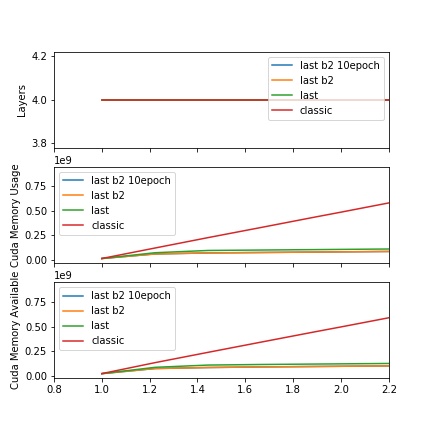
\includegraphics{parts/appendix/reports-gmsnn/docs_esteban-latex/test_reports/2018-06-12/history_memory_1e.png}
\caption{Memory 1 epoch}
\end{figure}

\begin{figure}[h]
\centering
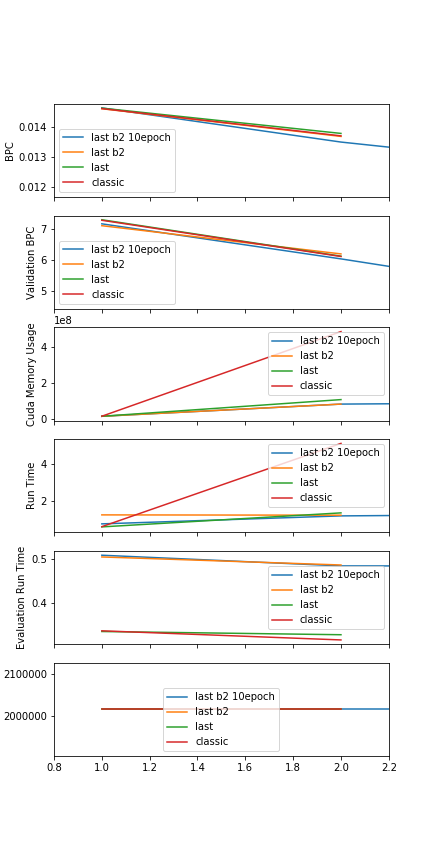
\includegraphics{parts/appendix/reports-gmsnn/docs_esteban-latex/test_reports/2018-06-12/history_frac_1e.png}
\caption{All info 1 epoch}
\end{figure}

\subsubsection{Results (full)}

\begin{figure}[h]
\centering
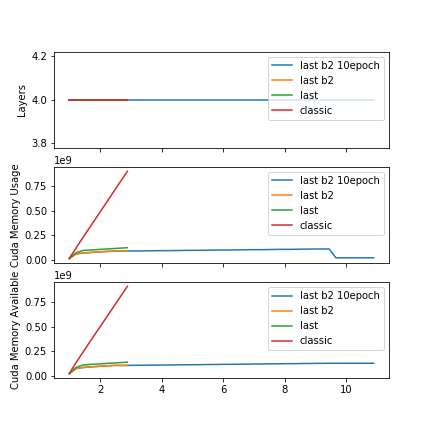
\includegraphics{parts/appendix/reports-gmsnn/docs_esteban-latex/test_reports/2018-06-12/history_memory.png}
\caption{Memory}
\end{figure}

\begin{figure}[h]
\centering
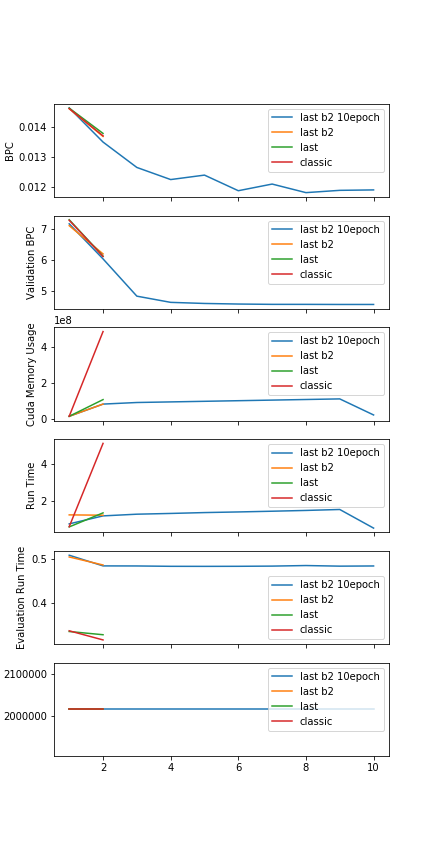
\includegraphics{parts/appendix/reports-gmsnn/docs_esteban-latex/test_reports/2018-06-12/history_frac.png}
\caption{All info}
\end{figure}

\paragraph{\texorpdfstring{Ram consumption for ``last b2 10epoch''}{Ram consumption for last b2 10epoch}}

\begin{figure}[h]
\centering
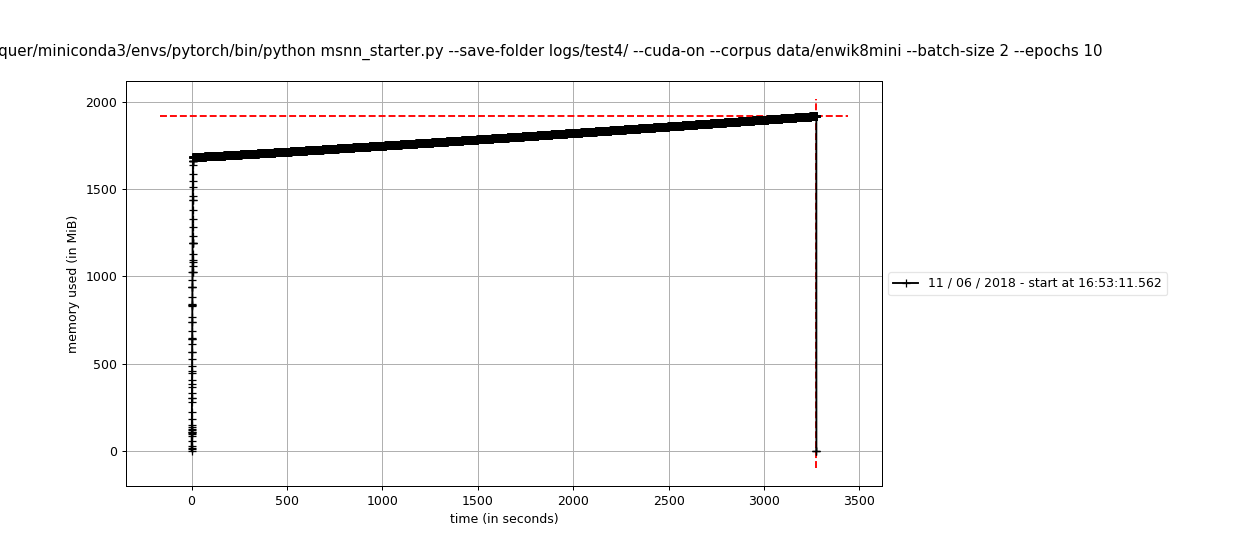
\includegraphics{parts/appendix/reports-gmsnn/docs_esteban-latex/test_reports/2018-06-12/history_RAM.png}
\caption{RAM 10 epoch}
\end{figure}

\subsection{Conclusion}

\subsubsection{Memory leak}

The leak in CUDA memory has reduced drastically.

It seems there is still a leak, this leak is not present when CUDA is
not used. This leak is present in both RAM and graphical RAM, but the
remaining leak in graphical RAM is not a concern anymore, with only a
dozen MiB over 1,000,000 characters (10 epochs * 100,000 characters).
However, the leak in RAM has not reduced, and even if it is not a
problem thanks to the available RAM in the cluster, it would be
preferable to identify the source of the leak.

\subsubsection{Run (training) time}

Additionally, the correlation of CUDA memory usage and and training run
time is kept, so the small remaining CUDA leak is probably linked to the
computation graph. With CUDA memory usage drastically reduced, run time
has been reduced too.

Currently, training over 100,000 characters (with 2 batches) only takes
5 minutes.

\subsubsection{Performances}

No conclusion can be drawn on learning performances, due to the size of
the learning corpus. Even though, it is encouraging that even with a
small corpus 10 epochs are not enough to have over-fitting (at least
with 2 batches).

\subsection{Next steps}

\begin{enumerate}
\def\labelenumi{\arabic{enumi}.}
\item
  long training over the ``enwik8reduced'' or the ``enwik8'' corpus;
\item
  fix (or at least identify) RAM leak
\end{enumerate}
